%================================================================
% UNIVERSIDADE FEDERAL DE UBERLÂNDIA
% FACULDADE DE MATEMÁTICA
% TEMPLATE PARA TRABALHOS ACADÊMICOS
% EVENTO: XIX SEMAT E IX SEMEST
% AUTOR: PROF. DR. ALESSANDRO ALVES SANTANA 
%================================================================
% DEFINIÇÃO DO TIPO DE DOCUMENTO
%================================================================
\documentclass[10pt]{article}
%================================================================
% TEMPLATE COM O CARREGAMENTO DOS PACOTES E DEMAIS CONFIGURAÇÕES
%================================================================
\usepackage{template-semat-semest-2019}
%================================================================
% DOCUMENTO PRINCIPAL
%================================================================
\begin{document}
\cabecalho
%================================================================
% TÍTULO DO TRABALHO
%================================================================
\titulo{Aplicações da Série de Taylor}
%================================================================
% AUTORIA DO TRABALHO
%
% DENTRO DO AMBIENTE autoria, O PRIMEIRO AUTOR(A) A SER INFORMADO
% É O AUTOR QUE IRÁ APRESENTAR E O ÚLTIMO SÃO AS INFORMAÇÕES DO 
% ORIENTADOR(A). SEGUE EXEMPLO ABAIXO   
% 
% \begin{autoria}{número de autores(as)}
%   
% \apresentador{nome completo do apresentador(a)/orientando(a)}
%  {instituição de origem do apresentador(a)/orientando(a)}
%  {unidade acadêmica da instituição de origem}
%  {e-mail do apresentador(a)}
%
% \orientando{nome completo do orientando}
%  {instituição de origem do orientando}
%  {unidade acadêmica da instituição de origem}
%  {e-mail do orientando(a)}
%
% \orientando{nome completo do orientando(a)}
%  {instituição de origem do orientando(a)}
%  {unidade acadêmica da instituição de origem}
%  {e-mail do orientando(a)}
%
% \orientador{nome completo do orientador(a)}
%  {instituição de origem do orientador(a)}
%  {unidade acadêmica da instituição de origem}
%  {e-mail do orientador(a)}
%
% \end{autoria}
%    
%================================================================
\begin{autoria}{3}

\apresentador{Studant Dezes Perado}
{Universidade Federal de Uberlândia}
{Faculdade de Matemática}
{studant.perado@ufu.br}

\orientando{Hopera Dorderi Wada}
{Universidade Federal de Uberlândia}
{Faculdade de Matemática}
{hopera.dorderi@ufu.br}

\orientador{Alge Brabu Leana}
{Universidade Federal de Uberlândia}
{Faculdade de Matemática}
{alge.leana@ufu.br}

\end{autoria}

%================================================================
% LEIA ATÉ O FINAL O QUE ESTÁ ABAIXO.
%================================================================
% PARA INSERIR TEOREMA, DEFINIÇÃO, LEMA OU COROLÁRIO USE O MODELO 
% ABAIXO. O MÉTODO DE INSERÇÃO PARA TEOREMA É
%
% \begin{teorema}{nome do teorema}{label(rótulo) do teorema}
%   Descrição do teorema
% \end{teorema}
%
% SE FOR UM COROLÁRIO,
%
% \begin{corolario}{nome do corolário}{label(rótulo) do corolário}
%   Descrição do colorário
% \end{corolario}
%
% SE FOR UM LEMA,
%
% \begin{lema}{nome do lema}{label(rótulo) do lema}
%   Descrição do lema
% \end{lema}
%
% SE FOR UMA DEFINIÇÃO
%
% \begin{definicao}{nome da definição}{label(rótulo) da definição}
%   Descrição da definição
% \end{definicao}
%
% IMPORTANTE:
% 
%  - SE O TEOREMA, COROLÁRIO, LEMA OU DEFINIÇÃO NÃO TIVER NOME 
%    COLOQUE AS CHAVES SEM NADA DENTRO. O MESMO VALE NO CASO DE 
%    NÃO HAVER RÓTULO, COLOQUE AS CHAVES SEM NADA DENTRO. 
%    POR EXEMPLO, UMA DEFINIÇÃO SEM NOME E RÓTULO, FICA ASSIM 
%     
%    \begin{definicao}{}{}
%     Descrição da definição
%    \end{definicao}
%
%  - SE FOR REFERENCIAR UM TEOREMA, NO TEXTO COLOQUE  
%    \ref{teo:nome do rótulo}. POR EXEMPLO:
%
%    \begin{teorema}{Teorema de Pitágoras}{pitagoras}
%     Em todo triângulo retângulo tendo $a$ como hipotenusa, 
%     sendo $b$ e $c$ seus catetos, vale a relação
%     \[ a^2=b^2+c^2.\]
%    \end{teorema}
%
%    PARA REFERENCIAR ESSE TEOREMA NO TEXTO BASTA COLOCAR  
%    \ref{teo:pitagoras}. SE FORSSE UMA DEFINIÇÃO,  
%    USE \ref{def:rótulo da definição}. PARA COROLÁRIO E LEMA 
%    USE, RESPECTIVAMENTE, \ref{cor:rótulo do corolário} e
%    \ref{lem:rótulo do lema}.
%
%   - AO ROTULAR OS TEOREMAS, COROLÁRIO, LEMAS E DEFINIÇÕES, 
%     USE APENAS LETRAS MINÚSCULAS, SEM ACENTO E SEM ESPAÇO.
%    
%   - O MODELO ABAIXO APRESENTA UM EXEMPLO PARA TER COMO 
%     REFERÊNCIA.
% 
%================================================================

%\pagestyle{principal}

\section{Introdução}

A chamada \emph{série de Taylor} é uma forma de representação de funções. 
Esse tipo de série tem um grande número de aplicações. Uma das aplicações  
reside no desenvolvimento de métodos de resolução numérica para equações 
diferenciais. Em essência, desde que a função envolvida possua derivadas 
de qualquer ordem em um ponto de seu domínio, a série de Taylor representa 
essa função por meio de uma série de potências. Assim sendo, vamos 
primeiramente formalizar a série de Taylor pelo Teorema \ref{teo:taylor}.

\begin{teorema}{Fórmula da Série de Taylor com resto de Lagrange}{taylor}
Seja $f:[a,b]\rightarrow \mathbb{R}$ um função com $n$ derivadas contínuas 
e $f^{(n+1)}$ definida em todo intervalo $(a,b)$. Se $x_0\in[a,b]$, 
$\exists \varepsilon$ entre $x_0$ e $x$ tal que
\begin{equation}
f(x)=\sum\limits_{k=0}^{n}\dfrac{f^{(k)}(x_0)}{k!}(x-x_0)^k+
\dfrac{f^{(n+1)}(\varepsilon)}{(n+1)!}(x-x_0)^{n+1}.
\label{eq1}
\end{equation}
\end{teorema}

O Teorema de Taylor com Resto de Lagrange garante simplesmente que
existe uma função para o resto e que seu valor existe para algum 
número entre $x_0$ e $x$. A questão nesse ponto é que na maioria dos 
casos não é possível obter o valor de $\varepsilon$ para cada valor 
de $x$ que permita obter o erro. 

Observando ainda o teorema dado, se desprezarmos o resto, a série 
de Taylor é um polinômio de grau $n$ expresso, ao abrir a série, por
\[
f(x)=f(x_0)+f^{(1)}(x_0)(x-x_0)+\dfrac{f^{(2)}(x_0)}{2!}
(x-x_0)^2+\cdots+\dfrac{f^{(n)}(x_0)}{n!}
(x-x_0)^n
\]
e representa uma aproximação, com um determinado grau de precisão, 
para a função original $f(x)$, em uma região em torno de $x_0$ e 
quanto mais próximo de $x_0$ for a variável $x$, mais preciso será 
essa aproximação. Se observarmos a expressão do resto no teorema, 
pode se ver esse resto tende a zero quando $x$ tende a $x_0$. 
Além disso, ressalta-se que quanto maior for o valor de $n$ melhor é 
a aproximação. Para exemplificar, considere a expansão da função 
$f(x)=\cos(x)$, em termos de série de Mac-Laurin 
(que é caso quando $x_0=0$) até $n=8$, a qual é dada abaixo.
\begin{equation}
f(x)=1-\frac{{{x}^{2}}}{2}+\frac{{{x}^{4}}}{24}-
\frac{{{x}^{6}}}{720}+\frac{{{x}^{8}}}{40320}
\end{equation}
A Fig. \ref{fig1} apresenta o gráfico da função $f(x)=\cos(x)$ e as demais 
figuras os gráficos desta juntamente com os polinômios de Taylor de 
graus 2, 4, 6 e 8 no intervalo $[-6,6]$.

\begin{figure}[H]
\centering
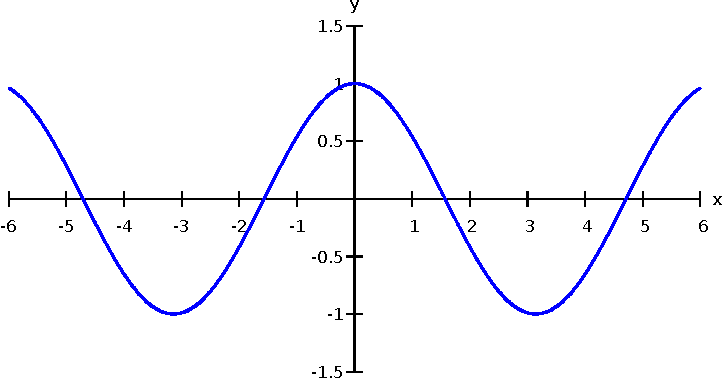
\includegraphics[scale=1]{fx.pdf}
\caption{Gráfico da função $f(x)=\cos(x)$}
\label{fig1}
\end{figure}

\begin{figure}[H]
\begin{minipage}[t]{0.45\textwidth}
\centering
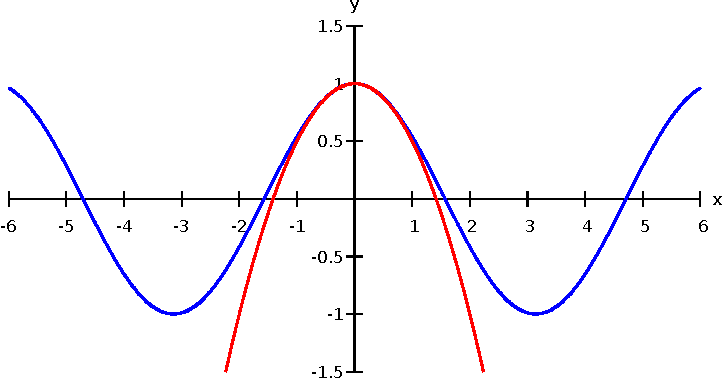
\includegraphics[scale=0.68]{fx-px2.pdf}
\caption{Função $f(x)=\cos(x)$ com $p_2(x)$.}
\label{fig2}
\end{minipage}%
\hfill
\begin{minipage}[t]{0.45\textwidth}
\centering
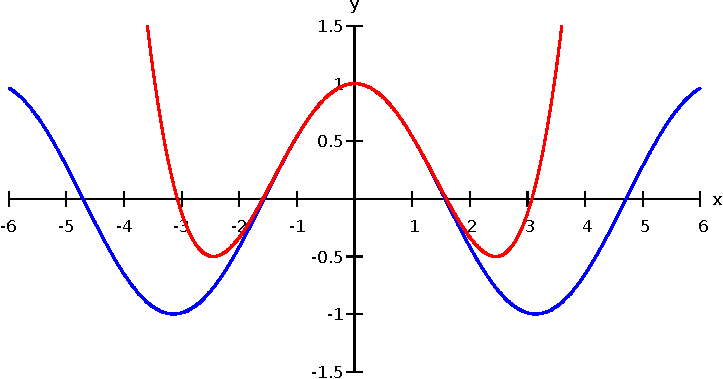
\includegraphics[scale=0.68]{fx-px4.pdf}
\caption{Função $f(x)=\cos(x)$ com $p_4(x)$.}
\label{fig3}
\end{minipage}
\end{figure}

\begin{figure}[H]
\begin{minipage}[t]{0.45\textwidth}
\centering
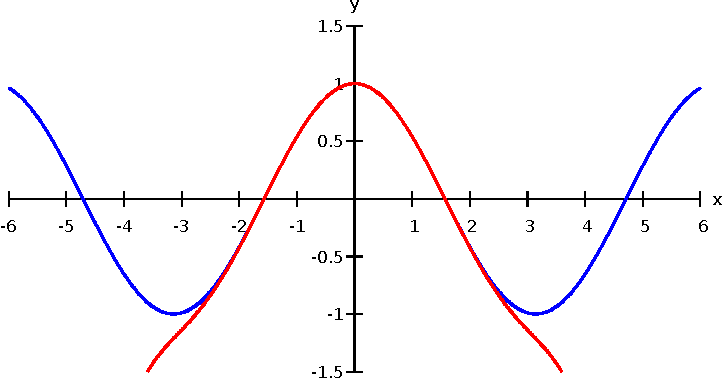
\includegraphics[scale=0.68]{fx-px6.pdf}
\caption{Função $f(x)=\cos(x)$ com $p_6(x)$.}
\label{fig4}
\end{minipage}%
\hfill
\begin{minipage}[t]{0.45\textwidth}
\centering
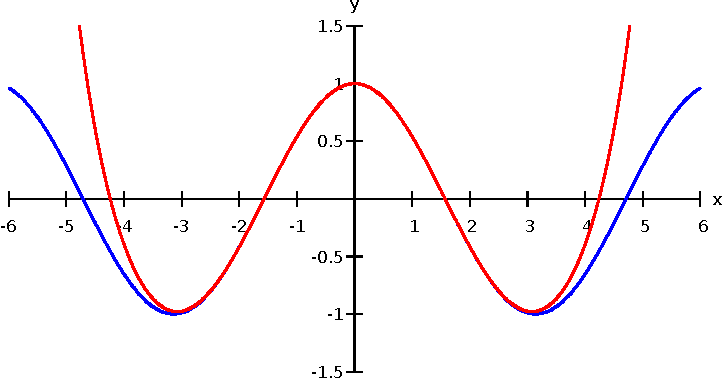
\includegraphics[scale=0.68]{fx-px8.pdf}
\caption{Função $f(x)=\cos(x)$ com $p_8(x)$.}
\label{fig5}
\end{minipage}
\end{figure}
Pode-se observar que o aumento do grau do polinômio de Taylor 
faz com que o polinômio se ajuste sobre a função $f(x)=\cos(x)$. 
Assim sendo, quando $n\rightarrow +\infty$ temos que 
$p_n(x)\rightarrow f(x)$.

Nas seções a seguir serão apresentadas algumas aplicações da Série 
de Taylor.
 
\section{Cálculo de aproximações de integrais}

Não é possível obter analiticamente a primitiva da maioria das integrais que 
aparecem em situações práticas. A série de Taylor pode ser empregada para 
obter aproximações de integrais definidas onde o integrando não pode ser 
integrado analiticamente. Assim sendo, para exemplificar, vamos obter uma 
aproximação para a integral da função $f(x)=e^{-x^2}$ no intervalo 
$[-1,1]$, ou seja, vamos calcular a integral definida
\begin{equation}
\int\limits_{-1}^{1}\,e^{-x^2}\,dx
\label{integral}
\end{equation}   
aproximando $f(x)=e^{-x^2}$ por uma série de Taylor, em torno de $x=0$, 
e integrar o polinômio gerado pela série de Taylor no intervalo $[-1,1]$. 
Considerando o polinômio de Taylor de grau 2 para aproximar 
$f$, temos que
\begin{equation*}
f(x)\approx \sum\limits_{k=0}^{2}\,\dfrac{f^{(k)}(a)}{k!}
\Rightarrow
f(x)\approx f(0)+f^{(1)}(0)x+\dfrac{f^{(2)}(0)}{2}x^2.
\end{equation*}
As derivadas de primeira e segunda ordens de $f$ são, respectivamente,
\[ 
f^{(1)}(x)=-2xe^{-x^2}\;\;\text{e}\;\;f^{(2)}(x)=(4x^2-2)e^{-x^2}.
\] 
Avaliando essas derivadas em $x=0$, segue que $f^{(1)}(0)=0$ e 
$f^{(2)}(0)=-2$. Portanto, a aproximação de $f(x)$ por um polinômio de 
Taylor de ordem $2$ é 
\begin{equation*}
f(x)\approx 1-x^2.
\end{equation*}
Continuando,
\begin{equation*}
\int\limits_{-1}^{1}\,e^{-x^2}\,dx\approx 
2\int\limits_{0}^{1}\,(1-x^2)\,dx
\Rightarrow
\int\limits_{-1}^{1}\,e^{-x^2}\,dx\approx 2\left[x-\dfrac{x^3}{3}\right]
_{0}^{1}\Rightarrow \int\limits_{-1}^{1}\,e^{-x^2}\,dx\approx \dfrac{4}{3}. 
\end{equation*}

E com isso temos uma aproximação para a integral da função $f(x)=e^{-x^2}$ 
no intervalo $[-1,1]$. Ressalta-se que quanto mais termos tiver o polinômio 
gerado pela série de Taylor melhor vai ser a aproximação. 

\section{Fórmulas de diferenças finitas}

As chamadas \textbf{Fórmulas de Diferenças Finitas (FDF)} são fórmulas de 
aproximações para derivadas e tem uma grande aplicação no desenvolvimento 
de métodos de resolução numérica de EDO e EDP. 
O chamado \textbf{Método de Diferenças Finitas} 
é um método de resolução numérica de equações diferenciais que tem por 
base a aproximação das derivadas dessas equações por fórmulas de diferenças finitas. 
Essas fórmulas são obtidas utilizando expansões em série de Taylor da função 
incógnita. Vamos exemplicar isso obtendo uma fórmula de diferença finita 
para a derivada segunda de uma função $f$. Suponha que se tenha interesse em obter uma 
fórmula para aproximar a derivada segunda de uma função $f$ de tal forma que
\begin{equation}
f^{(2)}(x)=\alpha f(x-\Delta x)+\beta f(x)+\gamma f(x+\Delta x).
\label{fdf1}
\end{equation}

Expandindo $f(x-\Delta x)$ e $f(x+\Delta x)$ em torno de $x$, temos que
\begin{subnumcases}{}
f(x-\Delta x)=f(x)-\Delta x f^{(1)}(x)+\dfrac{\Delta x^2 f^{(2)}(x)}{2}-
\dfrac{\Delta x^3 f^{(3)}(x)}{6}+\dfrac{\Delta x^4 f^{(4)}(x)}{24}-\dots
\label{fdf2}\\[1em]
f(x+\Delta x)=f(x)+\Delta x f^{(1)}(x)+\dfrac{\Delta x^2 f^{(2)}(x)}{2}+
\dfrac{\Delta x^3 f^{(3)}(x)}{6}+\dfrac{\Delta x^4 f^{(4)}(x)}{24}+\dots
\label{fdf3}
\end{subnumcases}

Substituindo \eqref{fdf2} e \eqref{fdf3} em \eqref{fdf1}, segue que
\begin{multline}
f^{(2)}(x)=
\alpha
\left[
f(x)-\Delta x f^{(1)}(x)+\dfrac{\Delta x^2 f^{(2)}(x)}{2}-
\dfrac{\Delta x^3 f^{(3)}(x)}{6}+\dfrac{\Delta x^4 f^{(4)}(x)}{24}-\dots
\right]+
\beta f(x)+\\[1em]
\gamma 
\left[
f(x)+\Delta x f^{(1)}(x)+\dfrac{\Delta x^2 f^{(2)}(x)}{2}+
\dfrac{\Delta x^3 f^{(3)}(x)}{6}+\dfrac{\Delta x^4 f^{(4)}(x)}{24}+\dots
\right].
\label{fdf5}
\end{multline} 

Agrupando e colocando em evidência os termos que envolvem $f(x)$, $f^{(1)}(x)$ 
e $f^{(2)}(x)$, 
\begin{equation}
f^{(2)}(x)=
\left(\alpha+\beta+\gamma\right)f(x)+
\left(-\alpha+\gamma\right)\Delta x f^{(1)}(x)+
\left(\dfrac{\alpha}{2}+\dfrac{\gamma}{2}\right)\Delta x^2 f^{(2)}(x)+\dots.
\label{fdf6}
\end{equation}

Desprezando os termos que envolvem as derivadas de terceira ordem em diante, 
para determinar $\alpha$, $\beta$ e $\gamma$, temos que resolver o 
sistema linear
\begin{equation}
\begin{cases}
\begin{array}{rcrcrcc}
\alpha & + & \beta &  + & \gamma & = & 0\\[1em]
\alpha &   &       &  - & \gamma & = & 0\\[1em]
\alpha & & & + & \gamma & = & \dfrac{2}{\Delta x^2}	
\end{array} 
\end{cases}
\xrightarrow{\text{solução}}
\begin{cases}
\begin{array}{rcc}
\alpha & = & \dfrac{1}{\Delta x^2}\\[1em]
\beta  & = & -\dfrac{2}{\Delta x^2}\\[1em]
\gamma & = & \dfrac{1}{\Delta x^2}	
\end{array} 
\end{cases}
\end{equation}

Com esses valores obtemos a fórmula 
\begin{equation}
f^{(2)}(x)\approx \dfrac{f(x-\Delta x)-2f(x)+f(x+\Delta x)}{\Delta x^2}
\end{equation}
de aproximação para a derivada segunda da função $f(x)$, a qual pode ser 
empregada fornecendo o valor de $x$ e de $\Delta x$. Claro que para obter 
uma aproximação razoável para $f^{(2)}(x)$ o valor de $\Delta x$ tem que 
ser pequeno, entre $(0,10^{-2})$, por exemplo. 

\section{Contexto Histórico}
O conceito de um resistor com memória existia mesmo antes da publicação de Leon Chua sobre o memristor em 1971. Em 1960, o professor Bernard Widrow, da Universidade de Stanford, desenvolveu um novo elemento de circuito chamado "memistor". Assim, a resistência do memistor foi controlada pela carga. Memistors formaram os componentes básicos da arquitetura de rede neural chamada ADALINE (ADAptive Linear NEuron).

%% A STUDY OF MEMRISTOR
Em 1971, Leon Chua, propôs que deveria haver um quarto elemento de circuito passivo fundamental para estabelecer uma relação matemática entre $q$ e $\varphi$, que ele chamou de memristor (um portmanteau de memória e resistor) [Chua, 1971]. Chua previu que uma classe de memristores poderia ser realizada na forma de um dispositivo puro de estado sólido sem uma fonte de alimentação interna.

Em 2008, Williams e outros, da Hewlett Packard, anunciaram o primeiro dispositivo memristor fabricado [Strukov et al., 2008]. No entanto, um resistor com memória não é uma coisa nova. Se tomar o exemplo da memória não volátil, ela remonta a 1960, quando Bernard Widrow introduziu um novo elemento de circuito chamado memistor [Widrow et al., 1960]. O motivo para escolher o nome de memistor é exatamente o mesmo que o memristor, um resistor com memória. O memistor possui três terminais e sua resistência é controlada pela integral de tempo de um sinal de corrente de controle. Isso significa que a resistência do memistor é controlada pela carga. Widrow inventou o memistor como um elemento de memória eletrolítica para formar um

%==========================================================================================
% INSERÇÃO DA BIBLIOGRAFIA
%==========================================================================================
% OBSERVAÇÃO IMPORTANTE: AS REFERÊNCIAS BIBLIOGRÁFICAS, DE ACORDO COM O TIPO DE 
% REFERÊNCIA DEVE SER INSERIDO DENTRO DO AMBIENTE theblibliography CONFORME EXPLICADO 
% ABAIXO:
%
% - PARA LIVRO:
%
%   \bibitem{label} nomes dos autores , \emph{título do livro}, editora, volume, ano de publicação.
%
% - PARA ARTIGO EM JORNAIS CIENTÍFICOS:
% 
%   \bibitem{label} nomes dos autores , \emph{título do trabalho}, nome da revista, ano de publicação.
% 
% - PARA ARTIGO PUBLICADO EM ANAIS DE EVENTOS:
% 
%   \bibitem{label} nomes dos autores , \emph{título do trabalho}, nome do evento, nome dos anais, 
%    ano de publicação.
% 
% - PARA MONOGRAFIA DE GRADUAÇÃO, DISSERTAÇÃO DE MESTRADO OU TESE DE DOUTORADO:
% 
%   \bibitem{label} nome do autor , \emph{título do trabalho}, escrever aqui de foi monografia de
%   graduação, dissertação de mestrado ou tese de doutorado , sigla da instituição e da unidade acadêmica, 
%   ano da defesa.
% 
%  - PARA REFERÊNCIAS DE INTERNET:
%
%   \bibitem{label} Título do assunto do sítio eletrônico, endereço do sítio eletrônico, acessado: data de acesso.
%
%   Abaixo, no modelo, pode se observar cada um dos exemplos supracitados.
%
%==========================================================================================

\begin{thebibliography}{1} 
\bibitem{leithold} 
Louis Leithold , \emph{O Cálculo com Geometria Analítica}, Harbra , vol.2 , 1994.
\bibitem{doug} Doug Pagnutti e Carl Ollivier-Gooch, \emph{A generalized framework for 
high order anisotropic mesh adaptation}, Computers and Structures, 2009. 
\bibitem{rafael} Rafael Yuri Medeiros Barbosa e Alessandro Alves Santana, 
\emph{Resolução da Equação de Advecção Difusão Via Método 
dos Volumes Finitos Baseado em Reconstrução de Alta Ordem Santana}, XVIII Semana da Matemática e 
VII Semana da Estatística, Anais da SEMAT e SEMEST, 2018.
\bibitem{gabriel} Gabriel Marcos Magalhães, \emph{Resolução Numérica da Equação 
de Advecção-Difusão Bidimensional via Método dos Volumes Finitos em Malhas Não-Estruturadas 
usando um Método de Reconstrução de Alta Ordem}, monografia de graduação, UFU-FEMEC, 2016.
\bibitem{gaussiana} Gaussian Quadrature, \url{https://en.wikipedia.org/wiki/Gaussian_quadrature}, 
acessado: 21/06/2019.
\end{thebibliography}




\end{document}